\chapter{Rationale}\label{chap:rationale}

\section{Introduction}

The research project, titled "Overall Power Optimization for Thread-Based Wireless Network," is a child project within the broader MOOD-Sense initiative. The MOOD-Sense project employs IoT devices to detect and predict challenging behavior in dementia patients. The project aims to develop an early warning system combining sensors, artificial intelligence, and wireless communication to provide feedback for healthcare professionals and improve patient care and safety \cite{MOOD-Sense_Research}.

This child project focuses on optimizing the energy efficiency and performance of the wireless Thread network protocol utilized by different wireless sensors and various MOOD-Sense projects. By examining network parameters such as transmission power, correct device types, path loss, positions, RSSI Downlink, RSSI Uplink, and more, this project aims to determine the optimal configuration of these parameters.

This child project forms a Thread network and employs an algorithmic approach to optimize network parameters using the appropriate hardware. The goal is to investigate how the transmission power parameter helps reduce the overall power consumption in an algorithmic approach while maintaining reliable communication between devices. Additionally, the project explores the integration of Thread with other wireless technologies, such as Bluetooth Low Energy, to enable connections between non-Thread-enabled devices.


\section{Problem Definition}
The growing reliance on wireless networks and IoT devices has intensified the need for energy-efficient communication protocols like Thread. Optimizing the energy efficiency and performance of the wireless Thread network protocol is essential for successfully operating various wireless sensors and applications. The challenge lies in determining the optimal configuration of network parameters, like transmission power and device types, to minimize power consumption without compromising reliability. Thread devices consume more power in mesh networks due to their high transmission frequency, leading to frequent battery replacement and reduced device availability. Furthermore, limited compatibility with existing devices can constrain Thread network protocol's functionality and reliability. Addressing these challenges is essential for realizing the full potential of Thread-based wireless communication in a wide range of fields.


\section{Goals and Objectives}
The main objective of this research project is optimizing power efficiency for the Thread network protocol, applicable in projects like MOOD-Sense. The research focuses on addressing power consumption and compatibility challenges, with the following goals:

\vspace{2mm}
\begin{enumerate}
    \item Examine the impact of transmission power optimization on Thread devices' power consumption.
    \item Apply algorithms like Monte Carlo and Genetic Algorithm for optimizing network parameters and determining efficient configurations.
    \item Evaluate optimized Thread network performance in various environments, comparing it to maximum power mode.
    \item Investigate integration with other wireless technologies, ensuring seamless communication with non-Thread devices.
    \item Suggest future research directions and improvements for Thread network optimization, including device positioning, path loss, and broader application scope.
\end{enumerate}
\vspace{3mm}


\section{Main Research Question}
\vspace{2mm}
\begin{itemize}
    \item How can parameter optimization be applied to develop a power-optimized Thread mesh wireless network?
\end{itemize}
\vspace{3mm}


\section{Sub-Research Questions}
\vspace{2mm}
\begin{enumerate}
    \item How does transmission power optimization affect Thread devices' power consumption?
    \item How can algorithms like Monte Carlo Method and Genetic Algorithm be applied to optimize network parameters and determine efficient configurations?
    \item How does optimized Thread network performance compare to maximum power mode in various environments?
    \item How can Thread be integrated with other wireless technologies to ensure seamless communication with non-Thread devices?
    \item What are the future research directions and improvements for Thread network optimization, including device positioning, path loss, and broader application scope?
\end{enumerate}
\vspace{3mm}


\section{Present Situation}
The MOOD-Sense research project had initially planned to use three wireless communication technologies, namely BLE, ZigBee, and WiFi, for the entire network communication. However, there has been no active implementation of any network protocol, and different subprojects are being carried out in parallel. These subprojects involve various aspects of the MOOD-Sense framework, such as the registration of dementia patient behavior and monitoring of the environmental context. However, the lack of a central network communication protocol has resulted in all the devices from different projects being separate, hindering data sharing and integration. The current state of the MOOD-Sense project can be visualized in the diagram, which shows the separate subprojects and devices without any active network implementation. The proposal to use a Thread mesh wireless network was introduced to address these issues due to its mesh nature, low cost, reliability, and remote management capabilities, making it an ideal candidate to connect BLE, ZigBee, and WiFi in a central place. The Thread mesh network protocol will enable seamless connectivity, interoperability, and communication among all devices in the MOOD-Sense framework.

\begin{figure}[!htb]
    \centering
    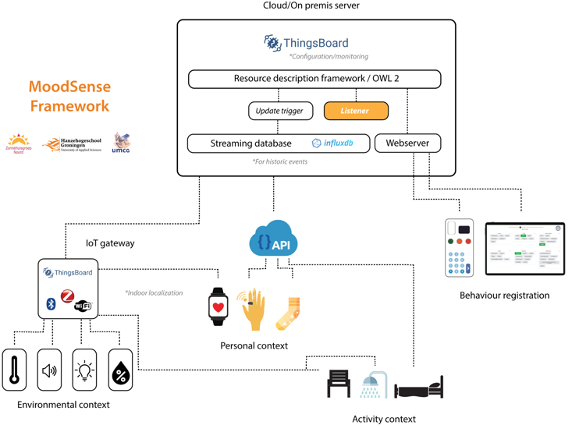
\includegraphics[width=0.8\textwidth]{images/rationale/rationale_present_situation.png}
    \caption{Current state of the MOOD-Sense project}
    \label{fig:rationale_present_situation}
\end{figure}


\section{Desired Outcome}
The desired outcomes of the current project aim to optimize the energy efficiency and performance of the wireless Thread network protocol while considering ethical aspects, reliable services, professional skills, applied research, and sustainability. The objective is to implement a Thread mesh network for seamless communication and to optimize power consumption through parameter optimization techniques, specifically transmission power. By comparing algorithmic approaches like Monte Carlo Method and Genetic Algorithm, the project seeks to identify the best method for achieving maximum power reduction while adhering to responsible research practices. Ultimately, the project aims to develop recommendations and strategies applicable to other MOOD-Sense projects, emphasizing ethical aspects, professional skills and applied research in developing and implementing energy-efficient wireless networks.
